% !TeX root = ../../thesis.tex
\chapter{In-Situ Annealing Effect on Morphology and Optical Properties}\label{ch:ellipsometry}


The GIWAXS measurements that were described in Chapter \ref{ch:material_properties} provided invaluable insights into the real-time annealing effect on thermally evaporated \ch{CsPbI2Br} thin films, including information about the phase transition temperatures, as well as the increase in crystallite size. However, GIWAXS is a rather complex and costly characterization technique, that requires access to synchrotron facilities, making it unsuitable for frequent and a lot characterization of samples. 

This is what gave the motivation to look for an alternative, in-house, characterization technique that could provide isnights into the real-time annealing effect on perovskite thin films. Necessary condtions would be to be compatible with the sof-nature of perovskite thin films, can be done in real time as annealing, and fast-enough acquisition time to detect real-time changes. 

Looking in literaute, temperature-dependent XRD is commonly used but there is al long time for each temperature point. Optical measurements like xx (from the paper) are usually associated with the developement of complex optical setups that create a large barrier with the measurement. 

In this chpater we demonstrate the use of Spectroscopic Ellipsometry when combined with a temperature stage, a fast, non-destructive optical characterization technique, that is commonly available in the vast majority of nano-electroni labs can be used to provide a wealth of information arounf the annealing effect both on the morpholgy and the otpical properties of the thin films. 
Initially, we lay the fundamentals aroung this caharacterization measurement, and introduce the experiment. Next, we delve into the dynamic model development which is the main innovation of the this shamber. In the last section we discuss the information we can extract about our film, including its expansion, grain coalesence, phase transitions. Additoianlly, we quantify relevant parameters like the Urbach energy and the thermo-optic coefficiet whic can be vital for the caracterization of the film. 




\section{Temperature-Dependent Spectroscopic Ellipsometry (SE)}


Spectroscopic ellipsometry (SE) is a widely used optical characterization technique, suitable for the determination of a thin film's thickness, roughness, optical constants, and more. Its working principle can be summarized as follows: 

\begin{enumerate}[i.]
  \item A linearly polarized light source is directed at a thin-film-coated substrate.
  \item The reflection and transmission of the incident light at the sample are governed by the Fresnel equations.
  \item The reflected light becomes elliptically polarized, meaning that the oscillatory directions of the electric field parallel (\textit{p}-plane) and perpendicular (\textit{s}-plane) to the incident plane are out of phase and have different amplitude.
  \item The reflected light gets detected by a polarization detection system.
\end{enumerate}

This change in polarization is described by two parameters, namely $\Psi$ and $\Delta$, which represent the amplitude ratio and phase difference between the p- and s-polarizations, respectively. This is summarized in equation: 

\begin{equation}
\frac{r_p}{r_s} = \tan(\Psi) \cdot e^{i\Delta},
\label{eq:ellipsometry}
\end{equation}

where $r_p$ and $r_s$ describe the reflection coefficient for the \textit{p}-polarized and \textit{s}-polarized light, respectively \cite{Fujiwara2018SpectroscopicCharacterization}.

SE data are typically collected across a wide range of wavelengths (300 nm - 2500 nm) and at various angles of incidence (between 45\degree and 85\degree). This relatively simple dataset contains ample information about the physical material properties of a thin film (including its thickness, roughness, dielectric functions, uniformity, composition, and more), however a careful model-based regression analysis is required to extrapolate them. This means that a model of the sample has to be created, which of consists of fixed and fitted parameters. Fixed parameters are the known samples properties (e.g. the dielectric function of the substrate), while fitted parameters are all the unknown properties that are under investigation. An initial "guessing" of these unknown properties is necessary, followed by an iterative data-fitting process that compares the simulated and experimental $\Psi$ and $\Delta$ values. In the end, the quality of the fitting process is described by the mean squared error (MSE), given by: 


\begin{equation}
\text{MSE} = \frac{1}{N - M} \sum_{i=1}^{N} \left[ \left( \frac{\Psi_{\text{meas},i} - \Psi_{\text{model},i}}{\sigma_{\Psi,i}} \right)^2 + \left( \frac{\Delta_{\text{meas},i} - \Delta_{\text{model},i}}{\sigma_{\Delta,i}} \right)^2 \right]
\label{eq:mse}
\end{equation}

where \( N \) is the number of data points, and \( M \) is the number of fitting parameters. The quantities \( \sigma_{\Psi,i} \) and \( \sigma_{\Delta,i} \) denote the standard deviation of each experimental data point. Typically, achieving an MSE that is as low as possible is the objective. In the framework of this study, an MSE below 20 is considered necessary to ensure a good match between experimental and simulated values. 


For the characterization of perovskite thin films via spectroscopic ellipsometry, the following protocol can be followed for a foolproof model development: 
\begin{itemize}
    \item The spectral range is limited to a region where the perovskite film is transparent, i.e. below its bandgap value. In the case of our thermally evaporated \ch{CsPbI2Br} thin films (\ch{E_g} = 645 nm), we limit the spectral range between 1000 and 2500 nm. 
    \item In this region, the extinction coefficient (k) of the material is equal to 0, so the response of the material can be solely described by its refractive index (n), via the empirical Cauchy dispersion model:
        \begin{equation}
            n(\lambda) = A + \frac{B}{\lambda^2} + \frac{C}{\lambda^4}
            \label{eq:cauchy}
        \end{equation}
    \item Besides the A, B, and C values of equation \ref{eq:cauchy}, additional fitting parameters include the thickness of the perovskite bulk and the thickness of the roughness layer (Fig. \ref{fig:ellipsometry:static_models}). The roughness is typically simulated as an additional layer, which follows the effective medium approximation (EMA), consisting of 50\% voids and 50\% the underlying material. 
    \item The raltively low number of fitting of paramters oft this model, as well as the small impact ofthe eroughness component in this region, make it ideal for a good approximation of the thickness of the perovskite thin film. 

\end{itemize}


\begin{figure}{}
  \centering
  \medskip
  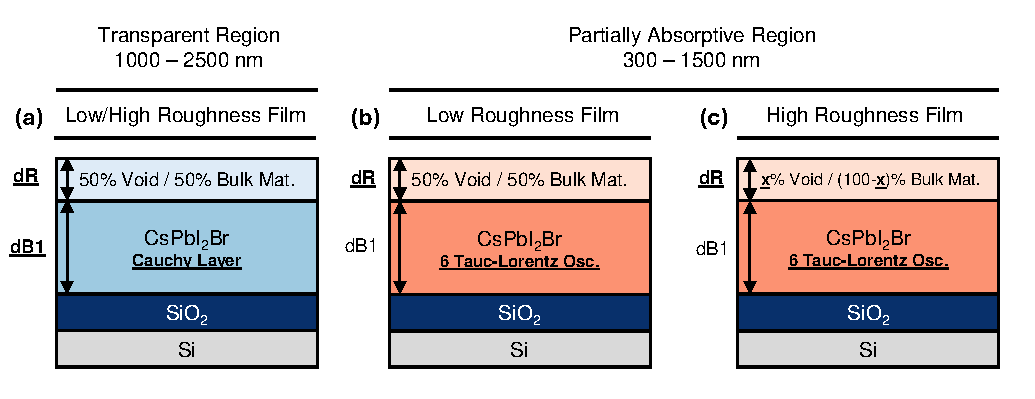
\includegraphics[width=.95\textwidth]{chapters/ellipsometry/image/Model_Approach.pdf}
  \caption{}
  \label{fig:ellipsometry:static_models}
\end{figure}




The properties of perovskite thin films have been widely studied by means of spectroscopic ellipsometry. It is an indispensable measurement for most labs, used to tune the fabrication process (via thickness estimations), extract the optical constants and use them for additional optical simulations, or extract relevant quality prameters (e.g. the Urbacj energy, bandgap, model the degradation of films 




 This measurments is typically done in the spectrun between 210 nm to 2500 nm. The perovskite is ablrorbing to part of this region and transpoarent to the rest. A common apporiach for the modeling is to rely on the tranparen region of the film, for the stimation og the thickness. Roughness dimension is much smaller than the wavelength and does not have as a strong impact, while sugan is refelcted from both the top and the bottom of the samples. For transparetn fimls, a simplified Cauchy model s typically used, which is described by the following formula. It is considered that the extinction ocefficient is 0 and that the refractive index is depednet onf the wavelenth through the formula xxxx. 

The modeling of the absorptinve region is vital for the estiamtion of the optical constants and the bandgap of the material. Oscillatior-based models that represent the oscialltors of the material. Many difference models are avaialble, namely Gaussian Oscialltors, Cody-Lorentz or Tauc-Lorents. The difference among lies on the xxx properties Short explanation of each model. 

In this work we opted for the use of Tauc Lorentz oscillators since they consider the xxx (see from book). 

It is possible to combine a temperatyre stage and peroforam the measuremetns as a fucntion of temp. This has been done previously for perovskite films and more. Most of times the results follow a step-wise increase in the temperature, stabilization, measurment, before increasing to the ext temperature step. However, we realized that this approach conceals infomration arounf the real time evolution of the effect, 

a static model has to be developed for eash static step which can be laborious, and there is also nocorrelation between two consecutuve measurements. 

For this reason, we decided to employ a continuoys heating ramp and obtain the Psi and Delta as a function of time and temperature, as shown in Fig. xx. the Psi and Delta give some high-level infomration about the period in the film that a lot of changes is happening, hoewegver needs to be modelled to further understand. The approach for the model mevelopement and the corroboration of the produed results will be firther duscussed in the next section. 

The appraoch for the development of this model will be described in the mext section.


\begin{itemize}
    \item Fundamentals of Spectroscopic Ellipsometry
    \item Room Temperature Characterization of Perovskite Thin Films
    \item Temperature-dependent works in literature
    \item Description of experiment
\end{itemize}

\subsection{SE Model Development}

Various Options were evaluated for the modelling of the temperatuer dependent results, according to literature and similar workds. 

The most straignht forward would be to split the time scale into smaller points and develop a spearates stac model for each of those. However, the loss of conintuoity might conseal real time information. 

The used software gives the option of dynamci modelling, that is the development of a model at t0, and the continuous fitting of its parameters to complete the whole time spectrum. We know that the thickness of the material is changing, the roughness is changeing (as shown formf the AFM pictures of the previous section) and also the position and intensituty of the oscillators is changing due to pahse changes, relaxatin of the badngap at high temperautres etc. This means that all the parametes of the thenitial model should be set as free (e.g. that is 24 parameters for the Tauch lorent + thickness + roughness). The continuous fitting of these paramters, is likely to lead to over-fitting behavior and the loos of physical meaning in the results. An example of thethickess an roughness evolution sis shown in Fig. xx, where abript changes in thickness and roughness are observed with little to no-physical meaning. 

Then there is a dynamic moelling development that was insipred for films SiGe. Whst wash shown is that they can develop a mmodel for specific stoichioemtries (E.G. XX ) and then describe the intermediate stoichiometris as superposition of the closests ones. 

we therfore realzed that we describe the material as a superpositions for a few static states that are slowly changing from one to the other. 

This positions were sected from careful consideration of he film. 

Moments t0 and t23 describe the initial and final state of the film, while t11 consisders the condition of the film at the higherst 300C (e.g. higher thickness due to expansion). psi and dlta reveal slo to changes happening between the 4th and the 8th minute of the epxriemetnt, threfore we develop an additional model for these two states to account for these cahnges. As it will be further discussed, these 5 models will be sufficient from the description fo the whole evolution of the film. 

Nedd to develop the 5 static models and corroborate their accuracy. 
This is more easily accessible for the models at t0 and t23, since we can do aadditional measuremmetns bfore and after the cahracterization of the film. 

\subsection{Development and Corroboration of Static Models}

Developing a model for the t0 is rather straight forward, due to the relatively low roughness of the film (RMS = 2, Fig. xx). Following the process desrcibed above, we use roughenss and mic of voids and below material we obtain athickness equal to xx nm, which id in good agreement with the profilometry measusmtens. W e then shoft to the partially absorptive reions, between 300 and 700 nm. Use of 6 Tauc-Lorentz Oscillators, achieve a model with an MSE of 12. As a genral rule of thumb an MSE below 20 inidcates a good fit, event though the physicallity should always be evaluated. For this reason, we extract the optical constants of the film, and use them to simulate the absorptance and reflectance of the films accorind to the transfer materix method. Fllowiwe experiementally evaluate the same parametersk in the lab doing rt measuremetns, an calculatign the A throug the relationship A= 100 - R - T. fIG shows the comparison between experiemtnal and simulated values, which confirms the accuracy of the static model at t0. 

Moving to the model of t23 proves to conceal challenges due to the high roughness of th film.Specififaclly, if they same rocess as above it is not possible to obtain a good MSE. Howeve, it is possibelt ot od so if we set hte thickness as a fit paramter. follwoed, iti is nindeed possble to obtain  good MSE, however the thickness is no longer relaistc (the obtained value i 310 nm while the thickness through elliposmetry if xx nm) It is alo not physical to have athicker film at the asamte temrature, same or thinner in case with have the elimination of voids. Hoe

The cause of this challenge was identified to be the increase roughness of the film. Specifially, the use onf an 50:50 EMA model is recomneded only in ase the dimension of the roughness element is less that 0.1 of the wavlenfth. This is in order to prevent sattering phenomena. The shotes wavelgnth we use of 300 nm, so the llargest roughness we culd have is 30 nm. This is close to the limiti of the EM model. In case, a larged discrepancy was observed it would be necessary to to use a multilayer approach, where the roughness is explained as a mulilayer EMA with variuous peroventages. 

However, since fo thsi type of example, the condition is cloe to the limit, we realized that is ti sposble ot fix the thickness and set the percentage of voids as a fitting paremeter. INdeed, with this simple adjustment it is possible to achieve both a good MSE and a relaisitc value of the thickness. The additional compariosn with the RT values as it was described above, furthe confirms the accuracy of the modelling approach. Th percentegae of voids was found to be close to 15\% for this pparoach. Therefore, we suse the same strategy ofr hte development of the additonal models at t5 t7 and t11. 


\subsection{Dynamic Model Developent}

We followngly use the 5 static models to develop the dynamic one. 
THe model is illustrated in figure xx. It is an EMA consisteing the 5 individal models. The paramters of these modelsa re fixed, the olume fraction si the fitted. An additioanl fitting parameter is the thickness o ht film so as to eplain the expansion, as well as the tickness of hte rouhness layer to try to indentify the changes in roughess and grain coalesence. We fit in real time. Fig xx shoes the evolution of the MSE as a function of time and tmperature, it mostly maintened below 20 which a first strong indication abotu the accuracy of the developed model. The following chapters will further examine the changes in the morphology of the otpical proporties og trhi films, drwaing comparison with additional in situ and ex situ characterization measurements. 

There are two types of scatter points the red is the model we describe above, the blue scatter points is a simplered causcy-based model that is only applied to the trnspoarent region. less sensitive to roughness variations, we use it as an additional control step to verify the peroformance of the dynamic model in the partially absorptive region. Both models are mainly absorbed below 20 MSE which si a first good sign for the accuracy. 


\begin{figure}[htbp]
    \centering
    % First plot
    \begin{subfigure}[t]{0.95\textwidth} % Adjust width if needed
        \centering
        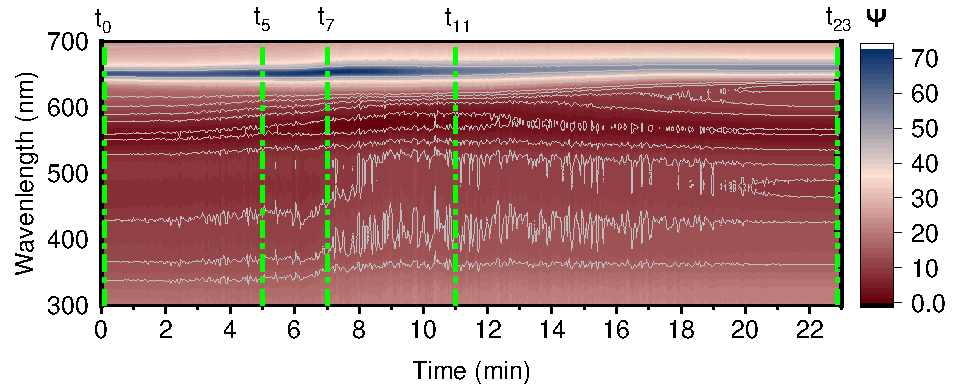
\includegraphics[width=\textwidth]{chapters/ellipsometry/image/Psi_Contour - MRS.pdf} % Replace with your image
        %\caption{Description for subplot (a).}
        %\label{fig:sub-a}
    \end{subfigure}

    \vspace{1em} % Space between the rows

    % Second plot
    \begin{subfigure}[t]{0.95\textwidth} % Adjust width if needed
        \centering
        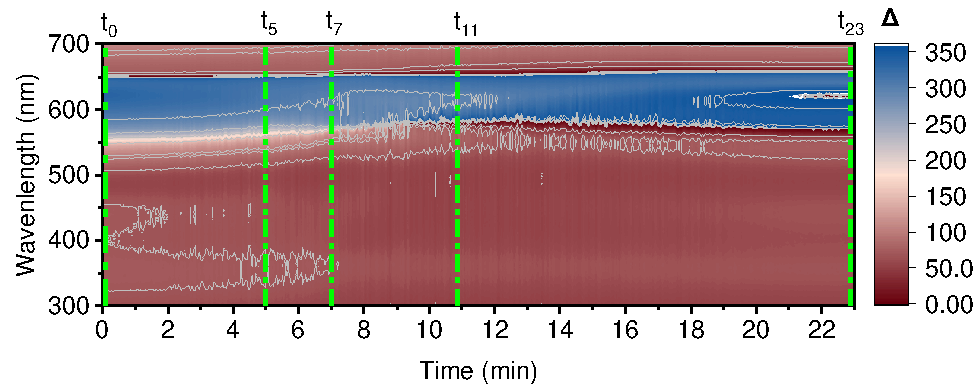
\includegraphics[width=\textwidth]{chapters/ellipsometry/image/Delta_Contour - MRS.pdf} % Replace with your image
        %\caption{Description for subplot (b).}
        %\label{fig:sub-b}
    \end{subfigure}

    % Caption for the whole figure
    \caption{}
    \label{fig:ellipsometry:raw_psi_delta}
\end{figure}





\begin{figure}[htbp]
    \centering
    % First row
    \begin{subfigure}[t]{0.45\textwidth}
        \centering
        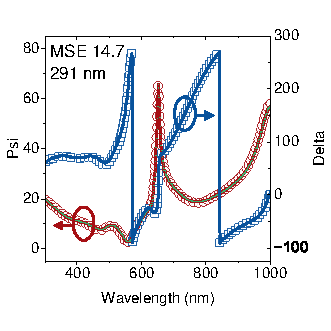
\includegraphics[width=\textwidth]{chapters/ellipsometry/image/t0_plot.pdf} % Replace with your image file
        \caption{As-Deposited State}
        \label{fig:ellipsometry:static_fits:t0}
    \end{subfigure}
    \hfill
    \begin{subfigure}[t]{0.45\textwidth}
        \centering
        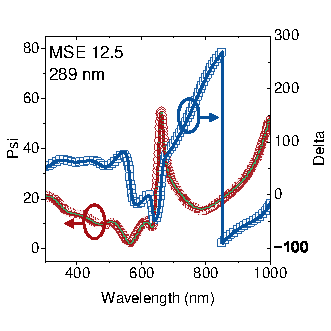
\includegraphics[width=\textwidth]{chapters/ellipsometry/image/t23_fixed_thick_x_void_p.pdf} 
        \label{fig:ellipsometry:static_fits:t23_fixed_thick_x_void}
        % Replace with your image file
        \caption{Annealed State - Model A}
    \end{subfigure}

    %\vspace{1em} % Space between rows

    % Second row
    \begin{subfigure}[t]{0.45\textwidth}
        \centering
        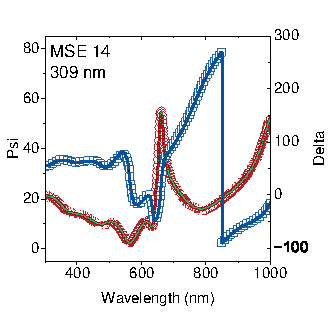
\includegraphics[width=\textwidth]{chapters/ellipsometry/image/t23_fitted_thickness.pdf} % Replace with your image file
        \caption{Annealed State - Model B}
        \label{fig:ellipsometry:static_fits:t23_fitted_thick}
    \end{subfigure}
    \hfill
    \begin{subfigure}[t]{0.45\textwidth}
        \centering
        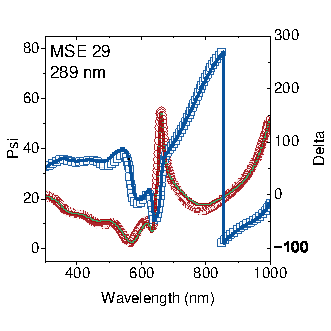
\includegraphics[width=\textwidth]{chapters/ellipsometry/image/t23_fixed_thickness_50_v.pdf} % Replace with your image file
        \caption{Annealed State - Model C}
        \label{fig:ellipsometry:static_fits:t23_fixed_thick_50_void}
    \end{subfigure}
    \caption{}
    \label{fig:ellipsometry:static_fits}
\end{figure}


\begin{figure}[htbp]
    \centering
    % First row
    \begin{subfigure}[t]{0.4\textwidth}
        \centering
        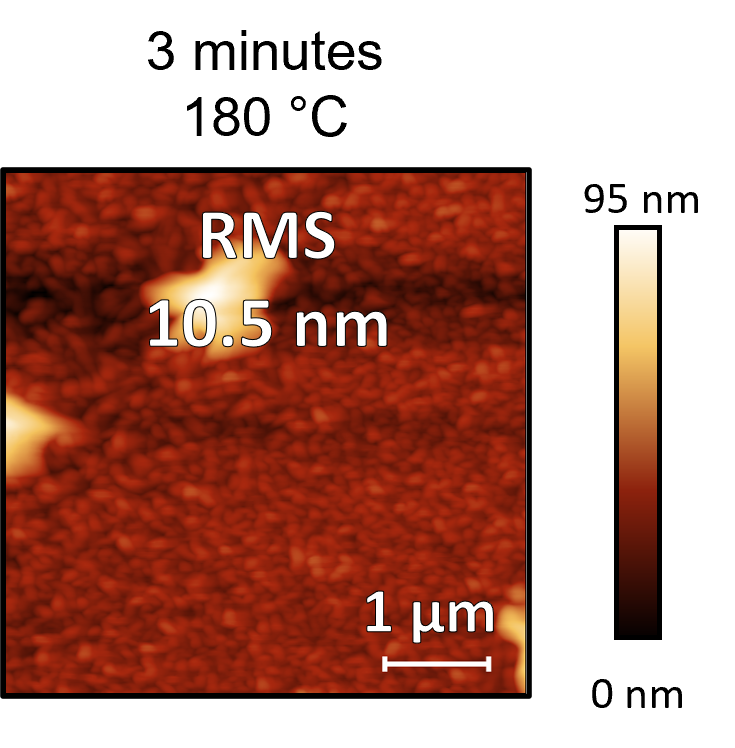
\includegraphics[width=\textwidth]{chapters/ellipsometry/image/180C_3min.png} % Replace with your image file
        \caption*{(a)}
    \end{subfigure}
    \hfill
    \begin{subfigure}[t]{0.4\textwidth}
        \centering
        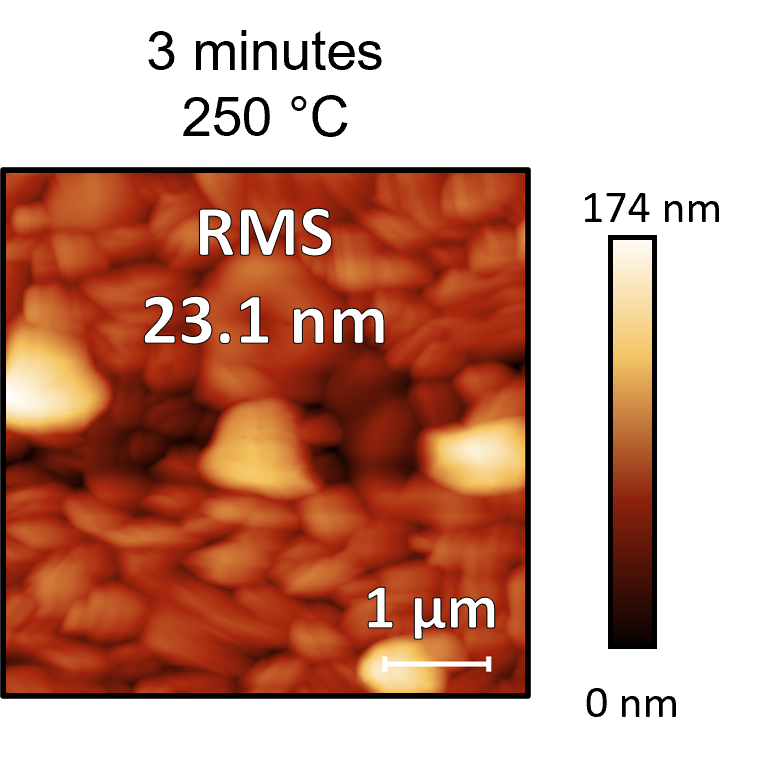
\includegraphics[width=\textwidth]{chapters/ellipsometry/image/250C_3min.png} % Replace with your image file
        \caption*{(b)}
    \end{subfigure}

    \vspace{1em} % Space between rows

    % Second row
    \begin{subfigure}[t]{0.4\textwidth}
        \centering
        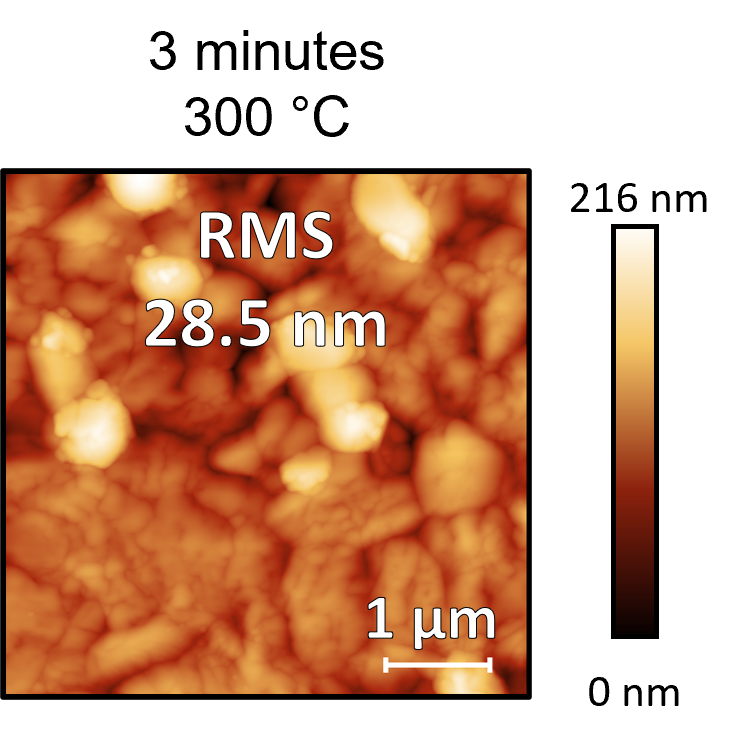
\includegraphics[width=\textwidth]{chapters/ellipsometry/image/300C_3min.png} % Replace with your image file
        \caption*{(c)}
    \end{subfigure}
    \hfill
    \begin{subfigure}[t]{0.4\textwidth}
        \centering
        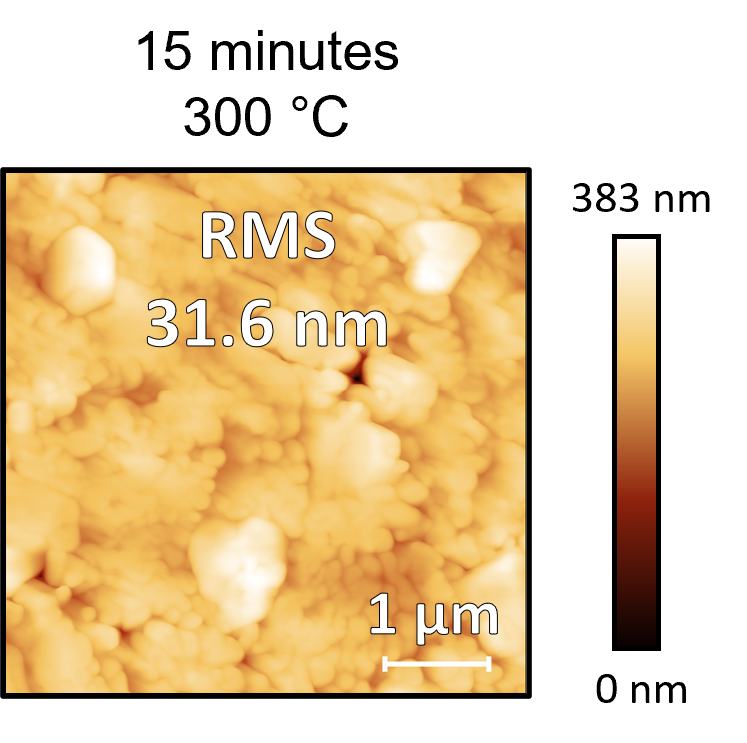
\includegraphics[width=\textwidth]{chapters/ellipsometry/image/300C_15min.png} % Replace with your image file
        \caption*{(d)}
    \end{subfigure}
    \caption{}
\end{figure}





\begin{figure}
  \centering
  \medskip
  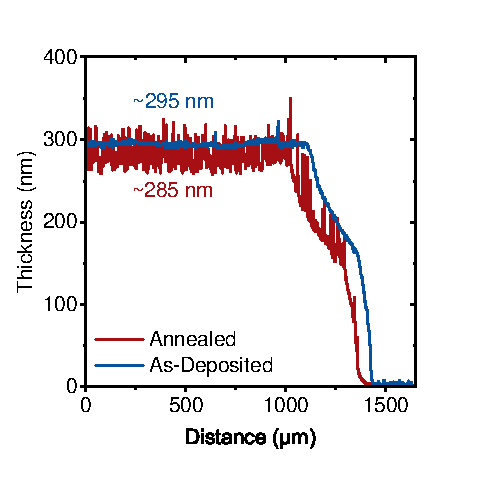
\includegraphics[width=.5\textwidth]{chapters/ellipsometry/image/Dektak.pdf}
  \caption{}
  \label{fig:ellipsometry:profilometry}
\end{figure}



\begin{figure}
  \centering
  \medskip
  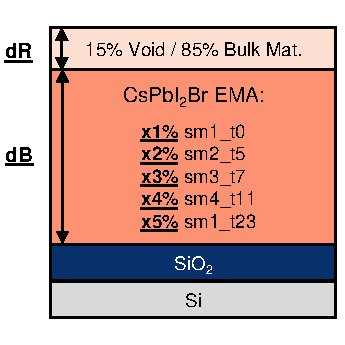
\includegraphics[width=.45\textwidth]{chapters/ellipsometry/image/Dynamic_Model.pdf}
  \caption{}
  \label{fig:ellipsometry:dynamic_model}
\end{figure}



\section{Results and Discussion}

\begin{figure}
  \centering
  \medskip
  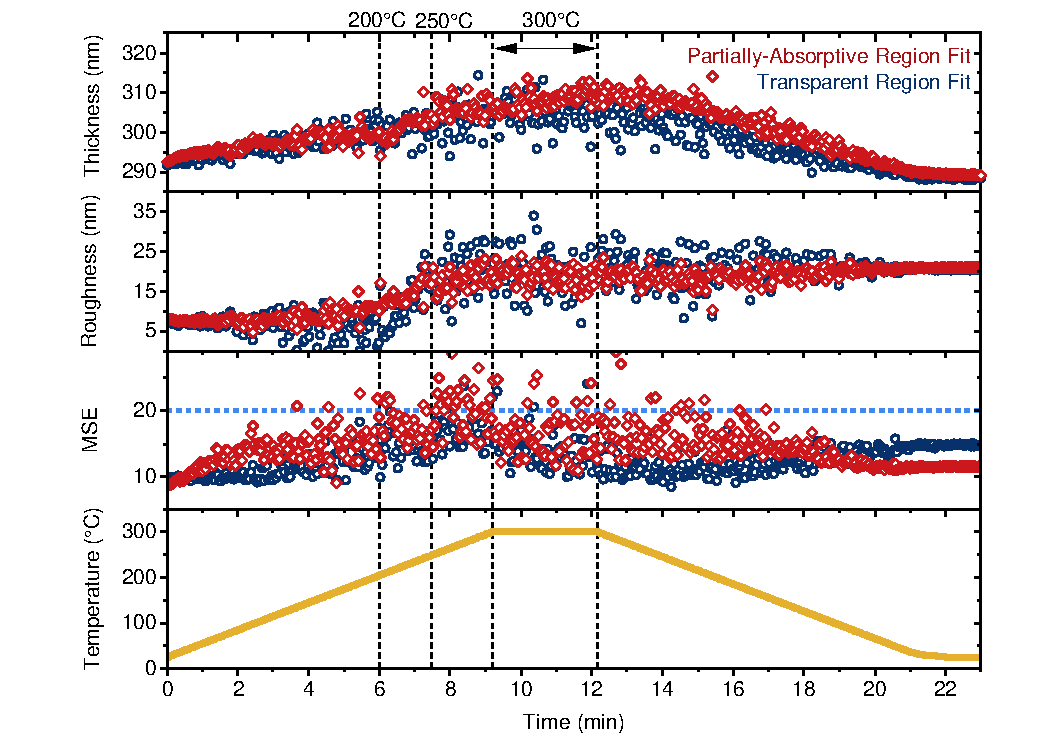
\includegraphics[width=.99\textwidth]{chapters/ellipsometry/image/Roughness_Thickness.pdf}
  \caption{}
  \label{fig:ellipsometry:roughness_thickness}
\end{figure}


\subsection{Thickness}
\subsection{Roughness}
\section{In situ annealing annealing effect on Optical Constants}

\begin{figure}
  \centering
  \medskip
  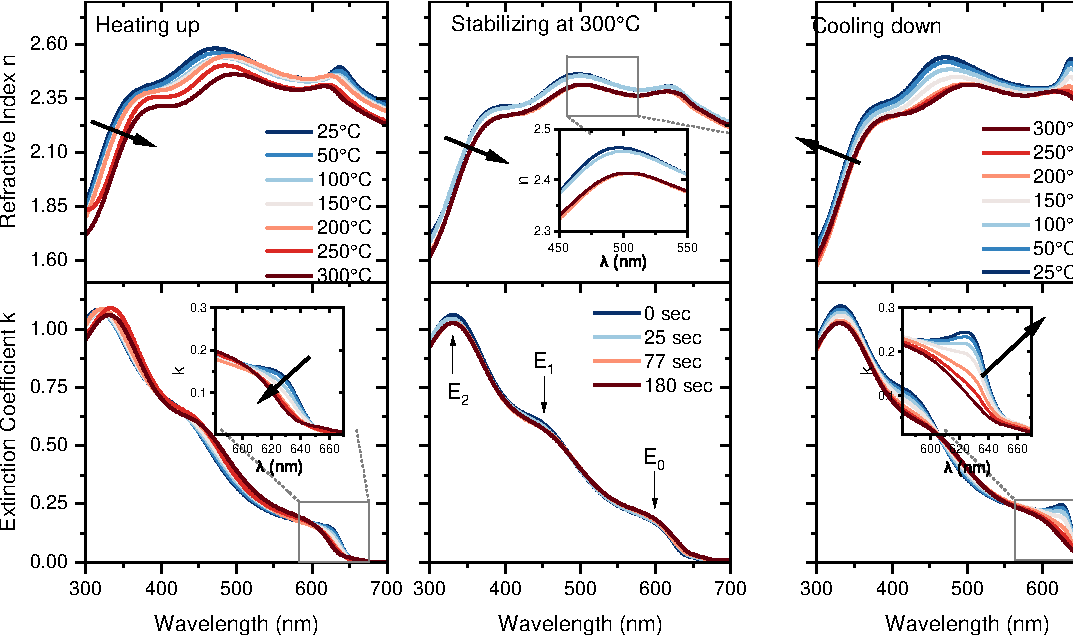
\includegraphics[width=.99\textwidth]{chapters/ellipsometry/image/Optical_constants.pdf}
  \caption{}
  \label{fig:ellipsometry:optical_constants}
\end{figure}


\subsection{Thermo-Optic Coefficient}

\begin{figure}[htbp]
    \centering
    \begin{subfigure}{0.32\textwidth}
        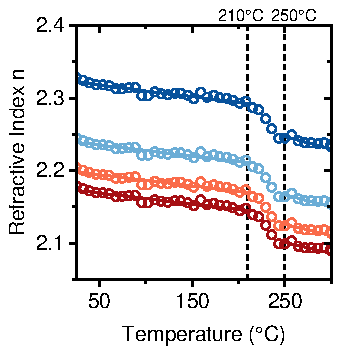
\includegraphics[width=\textwidth]{chapters/ellipsometry/image/Thermo-optic_Coefficient_heating.pdf}
        \caption{}
        \label{fig:ellipsometry:thermooptic_heating}
    \end{subfigure}
    \hfill
    \begin{subfigure}{0.32\textwidth}
        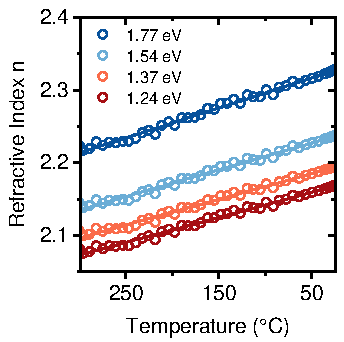
\includegraphics[width=\textwidth]{chapters/ellipsometry/image/Thermo-optic_Coefficient_cooling.pdf}
        \caption{}
        \label{fig:ellipsometry:thermooptic_cooling}
    \end{subfigure}
    \hfill
    \begin{subfigure}{0.3\textwidth}
        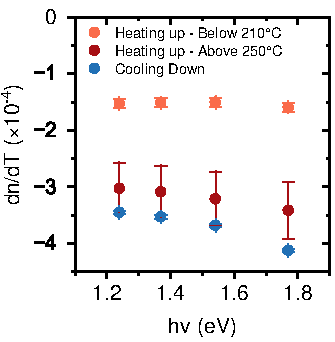
\includegraphics[width=\textwidth]{chapters/ellipsometry/image/Thermo-optic_Coefficient_energy.pdf}
        \caption{}
        \label{fig:ellipsometry:thermooptic_energy}
    \end{subfigure}
    \caption{A 1x3 figure layout.}
    \label{fig:ellipsometry:thermooptic}
\end{figure}



\subsection{Urbach Energy}

\begin{figure}[htbp]
    \centering
    \begin{subfigure}{0.32\textwidth}
        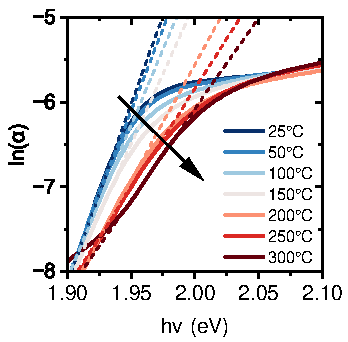
\includegraphics[width=\textwidth]{chapters/ellipsometry/image/Urbach_heating.pdf}
        \caption{}
        \label{fig:ellipsometry:urbach_heating}
    \end{subfigure}
    \hfill
    \begin{subfigure}{0.32\textwidth}
        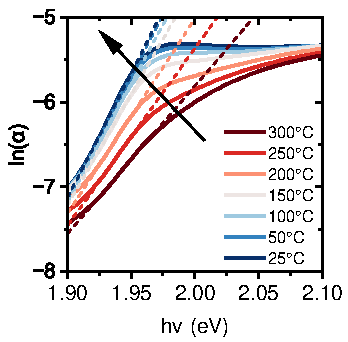
\includegraphics[width=\textwidth]{chapters/ellipsometry/image/Urbach_cooling.pdf}
        \caption{}
        \label{fig:ellipsometry:urbach_cooling}
    \end{subfigure}
    \hfill
    \begin{subfigure}{0.3\textwidth}
        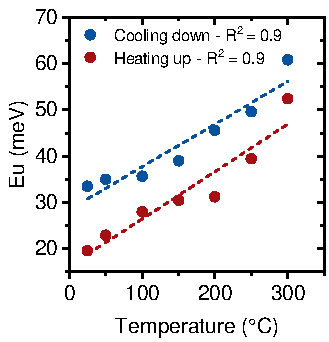
\includegraphics[width=\textwidth]{chapters/ellipsometry/image/Urbach_temp.pdf}
        \caption{}
        \label{fig:ellipsometry:urbach_temp}
    \end{subfigure}
    \caption{A 1x3 figure layout.}
    \label{fig:ellipsometry:urbach}
\end{figure}


\subsection{Critical Point Analysis}

\begin{figure}[htbp]
    \centering
    \begin{subfigure}{0.34\textwidth}
        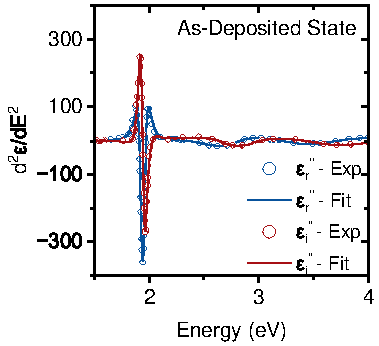
\includegraphics[width=\textwidth]{chapters/ellipsometry/image/Deriv_As_Dep.pdf}
        \caption{}
        \label{fig:ellipsometry:deriv:As_dep}
    \end{subfigure}
    \hfill
    \begin{subfigure}{0.31\textwidth}
        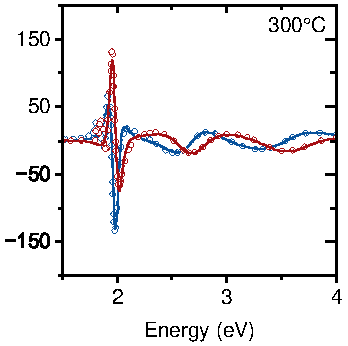
\includegraphics[width=\textwidth]{chapters/ellipsometry/image/Deriv_300C.pdf}
        \caption{}
        \label{fig:ellipsometry:deriv:300}
    \end{subfigure}
    \hfill
    \begin{subfigure}{0.31\textwidth}
        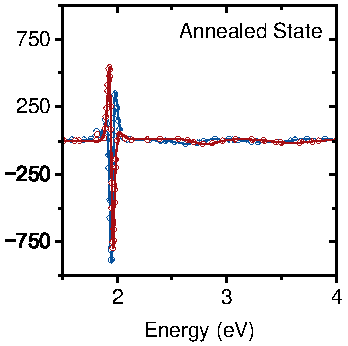
\includegraphics[width=\textwidth]{chapters/ellipsometry/image/Deriv_Anneal.pdf}
        \caption{}
        \label{fig:ellipsometry:deriv:anneal}
    \end{subfigure}
    \caption{A 1x3 figure layout.}
    \label{fig:ellipsometry:deriv}
\end{figure}

\begin{figure}[htbp]
    \centering
    \begin{subfigure}{0.34\textwidth}
        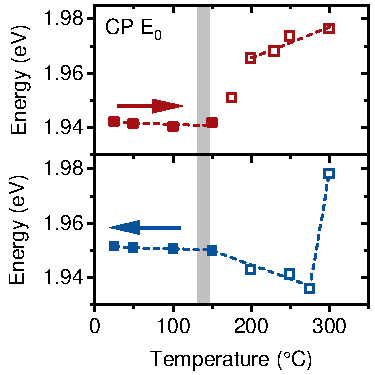
\includegraphics[width=\textwidth]{chapters/ellipsometry/image/CP0.pdf}
        \caption{}
        \label{fig:ellipsometry:CP0}
    \end{subfigure}
    \hfill
    \begin{subfigure}{0.31\textwidth}
        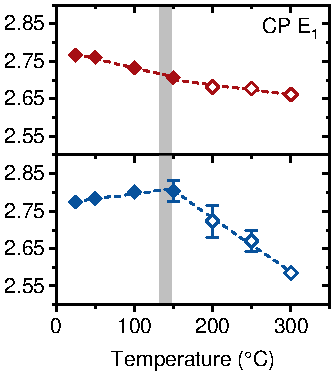
\includegraphics[width=\textwidth]{chapters/ellipsometry/image/CP1.pdf}
        \caption{}
        \label{fig:ellipsometry:CP1}
    \end{subfigure}
    \hfill
    \begin{subfigure}{0.31\textwidth}
        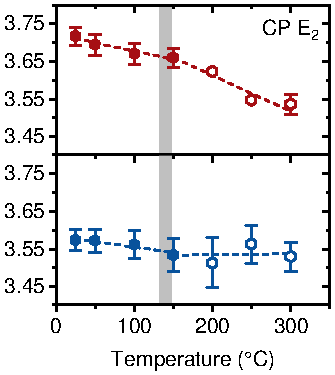
\includegraphics[width=\textwidth]{chapters/ellipsometry/image/CP3}
        \caption{}
        \label{fig:ellipsometry:deriv:CP2}
    \end{subfigure}
    \caption{A 1x3 figure layout.}
    \label{fig:ellipsometry:CP_all}
\end{figure}



\section{Conclusions}


%%%%%%%%%%%%%%%%%%%%%%%%%%%%%%%%%%%%%%%%%%%%%%%%%%
% Keep the following \cleardoublepage at the end of this file, 
% otherwise \includeonly includes empty pages.
\cleardoublepage

